%!TEX root = ../main_article.tex

\section{Introduction}

Code search plays an important role in the software development process, which is an essential field of Software Engineering and studies the semantic similarity between natural language queries and program code. 	Recent years have witnessed a huge increment in source code. The statistic shows that more than 60 million new projects have been created only in 2020. Thus, code search engines can improve the development efficiency of program developers, enabling them to search for existing code or examples of some API (Application Programming Interface), instead of “rebuilding wheels”. 

As deep learning has grown by leaps and bounds in recent years, a number of methods have been proposed in code search. such as Recurrent Neural Network (RNN) based models (\citealp{DeepCS}), Convolutional Neural Network (CNN) based models (\citealp{CQIL, ShuaiX0Y0L20}), graph based models (\citealp{, GuCM21}), and Pretrained Language Models (PLMs) based models (\citealp{CodeBERT, CoCLR, GraphCodeBERT, UniXcoder}). 

From the view of PLMs, all of them have well performance in code search, with complex model architecture and advanced training techniques. However, PLMs often treat code search as a downstream task, which means researchers can pretrain a model with hybrid objectives and multiple program language code data, then fine-tune it in a specific program language for code search (\citealp{UniXcoder,CodeBERT,GraphCodeBERT}). Our empirical study shows that there might be a performance decline when fine-tuning with data in multiple languages. Table~\ref{tab:comparison} shows MRR comparisons between single program language fine-tuned models and multiple program language fine-tuned models. Compared with multilingual models, code information can be roughly divided into identifier information, which distinguishes code from another code written in different program languages, and sentiment information, which reveals its intention. In code search, code sentiment information is only needed, for it is matched with specific queries. Identifier information may confound model training and decrease performance when fine-tuning with multiple program language data.


\begin{figure}[htb]
	\centering
	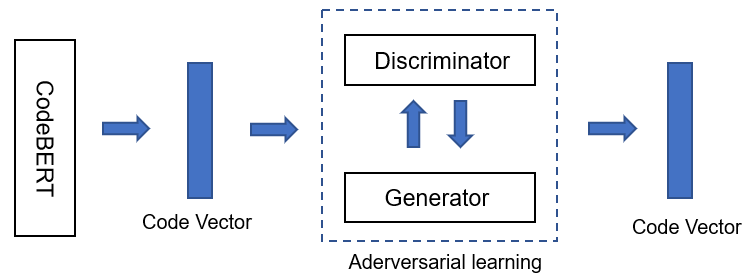
\includegraphics[width=1\linewidth]{imgs/structure.png}
	% \vspace{-15pt}
	\caption{Structure of the search enhancement framework.}
	% \vspace{-12pt}
	\label{fig:structure}
\end{figure}

Therefore, we want to reduce the identifier information of the embedding vector given by code search pre-trained models. We followed the idea of GANs (Generative Adversarial Networks, \citealp{goodfellow2020generative}) and propose a search enhancement framework. Our method consists of two additional networks: a generator, which aims to generate code search embedding vector with less identifier information, and a discriminator, of which the purpose is to identify the language feature. We treat the discriminator as a classification problem. When there is less identifier information, the discriminator may not classify the data well. Fig~\ref{fig:structure} illustrates our framework architecture.
In summary, our contributions are:
\begin{enumerate} 
\item Reveal the performance decline problem that appears when fine-tuning code search with multiple program languages.
\item We propose a search enhancement framework using GAN. It can reduce the identifier information of the embedding vector provided by code pre-trained networks, in order to focus the model on sentiment information.
\end{enumerate} 


% Table generated by Excel2LaTeX from sheet 'Sheet1'
\begin{table}[htbp]
	\centering
	\caption{Performance comparisons with different fine-tuning strategies}
	\vspace{-5pt}
	\resizebox{\linewidth}{!}{
	\begin{tabular}{lrrrr}
		\toprule
        & Python & Go  & Java & PHP \\
    \midrule
    Python & 0.369 & \_  & \_  &  \\
    Go  & \_  & 0.904 & \_  & \_ \\
    Java & \_  & \_  & 0.764 & \_ \\
    PHP & \_  & \_  & \_  & 0.708 \\
    Python\_Java & 0.468 & \_  & 0.708 & \_ \\
    Python\_Go & 0.404 & 0.882 & \_  & \_ \\
    Java\_Go & \_  & 0.902 & 0.724 & \_ \\
    Java\_PHP & \_  & \_  & 0.743 & 0.707 \\
    Java\_Python\_Go & 0.571 & 0.889 & 0.701 & \_ \\
    \bottomrule
	\end{tabular}%
	}
	\label{tab:comparison}%
	\vspace{-10	pt}
\end{table}%
